\section{Multivariable Functions}
\label{sec:multivariable-functions}

\subsection{Introduction}
Real life is rarely as simple as one input / one output. Many relationships depend on lots of variables. Here are some examples.
\begin{itemize}
  \item If I put a deposit into an interest-bearing account and let it sit, the amount I have at the end of three years depends on $P$ (how much my initial deposit is), $r$ (the annual interest rate), and $n$ (the number of compoundings per year).

  \item The air resistance on a wing in a wind tunnel depends on the shape of the wing, the speed of the wind, the wing's orientation (pitch, yaw, and roll), plus a myriad of other things that I can't begin to describe.

  \item The amount of your television cable bill depends on which basic rate structure you have chosen and how many pay-per-view movies you ordered.
\end{itemize}
Since the real world is so complicated, we want to extend our calculus ideas to functions of several variables.

\subsection{Functions of Two Variables}
If $x_1, x_2, x_3,\ldots, x_n$ are real numbers, then $(x_1,x_2,x_3,\ldots, x_n)$ is called an {\bf $n$-tuple}. This is an extension of ordered pairs and triples. A function of $n$ variables is a function whose domain\index{Domain} is some set of $n$-tuples and whose range\index{Range} is some set of real numbers.

For much of what we do here, everything will work the same whether we were working with 2, 3, or 47 variables. Because we're trying to keep things a little bit simpler, we'll concentrate on functions of two variables.

\begin{definition}[A Function of Two Variables]
A {\bf function of two variables}\index{Function}\index{Function!of two variables} is a function, that is, to each input is associated exactly one output.
    \begin{itemize}
    \item The inputs are ordered pairs, $(x,y)$.
    \item The outputs are real numbers (each output is a single real number).
    \item The domain of a function is the set of all possible inputs (ordered pairs);
    \item the range is the set of all possible outputs (real numbers).
    \item The function can be written $z=f(x,y)$.
    \end{itemize}
Functions of two variables can be described numerically (a table), graphically, algebraically (a formula), or in English.
\end{definition}
We will often now call the familiar $y=f(x)$ a {\bf function of one variable}\index{Function!of one variable}.

\begin{example}
The cost of renting a car depends on how many days you keep it and how far you drive. Represent this using a function.

\begin{solution} Let $d$ be the number of days you rent the car, and $m$ be the number of miles you drive. Then the cost of the car rental $C(d,m)$ is a function of two variables.
\end{solution}\end{example}

\begin{example}
The demand for hot dog buns depends on the price for the hot dog buns and also on the price for hot dogs. Represent this as a function.

\begin{solution} The demand $q_B=f(p_B,p_D)$ is a function of two variables. (The demand for hot dogs also depends on the price of both dogs and buns).
\end{solution}\end{example}

\subsection{Formulas and Tables}
Just as in the case of functions of one variable, we can display a function of two variables in a table. The two inputs are shown in the margin (top row, left column), and the outputs are shown in the interior cells.

\begin{example}
Table \ref{tab:4-1-rentcar} shows the cost $C(d,m)$ in dollars to rent a car for $d$ days and drive it $m$ miles.

\begin{table}[ht!]
\centering
    \begin{tabular}{*{5}{c}}
    $d$ & \multicolumn{4}{c}{$m$} \\
    \toprule
        & 100 & 200 & 300 & 400\\
    \midrule
    1   &  55 &  70 &  85 & 100\\
    2   &  95 & 110 & 125 & 140\\
    3   & 135 & 150 & 165 & 180\\
    \bottomrule
    \end{tabular}
    \caption{Cost, in dollars, to rent a car for $d$ days and drive $m$ miles.}
    \label{tab:4-1-rentcar}
\end{table}
\begin{enumerate}[label=(\alph*)]
    \item What is the cost to rent a car for 3 days and drive it 200 miles?

    \begin{solution}
    According to the table, renting the car for three days (row with $d=3$) and driving it 200 miles (column with $m=200$) will cost \$150.
    \end{solution}
    \item What is $C(100,4)$? What is $C(4,100)$?

    \begin{solution}
    Careful now -- the input is an ordered pair, so in $C(100,4)$, the 100 has to be a value of $d$ and the 4 has to be a value of $m$, so $C(100,4)$ would be the cost of renting a car for 100 days and driving it 4 miles. That cost is not in the table. (And that would be a pretty silly way to rent a car.) On the other hand, $C(4,100)$ is the cost of renting for 4 days and driving 100 miles. The table says that would cost \$175.
    \end{solution}
    \item Suppose we rent the car for three days. Is $C$ an increasing function with $d$ fixed at 3?

    \begin{solution}
If we know that $d$ is fixed at 3, we're looking at $C(3,m)$. This is now a function of one variable: just $m$. We can see the table that displays values of this function by focusing our attention on just the row where $d=3$.
\begin{table}[ht!]
\centering
    \begin{tabular}{*{5}{c}}
    $d$ & \multicolumn{4}{c}{$m$} \\
    \toprule
        & 100 & 200 & 300 & 400\\
    \midrule
    3   & 135 & 150 & 165 & 180\\
    \bottomrule
    \end{tabular}
\end{table}
Now we can see that if we rent for 3 days, the cost appears to be an increasing function of the number of miles we drive, which shouldn't be surprising.
    \end{solution}
\end{enumerate}
\end{example}

The idea of fixing one variable and watching what happens to the function as the other varies will come up again and again.

It's hard to display a function of more than two variables in a table. But it's convenient to work with formulas for functions of two variables, or as many variables as you like.

\begin{example}
The cost $C(d,m)$ in dollars to rent a car for $d$ days and drive it $m$ miles is given by the formula
$$C(d,m)=40d+0.15m \enspace .$$

\begin{enumerate}[label=(\alph*)]
    \item What is the cost of renting a car for 3 days and driving it 200 miles?

    \begin{solution}
     $C(3,200) = 40(3)+0.15(200)=\$150$. This is the same value we got from the table. The formula will give us the same answers for any of the table values.
    \end{solution}
    \item What is $C(100,4)$? What is $C(4,100)$?

    \begin{solution}
    $C(100,4)$ makes perfect sense to the formula (even if it doesn't make sense for actually renting a car). So now we can get an answer. To rent the car for 100 days and drive it for 4 miles should cost \$4000.60. $C(4,100)=\$175$, as before.
    \end{solution}
    \item Suppose we rent the car for three days. Is $C$ an increasing function with $d$ fixed at 3?

    \begin{solution}
    If we fix $d=3$, then $C(d,m)$ becomes $C(3,m)=40(3)+0.15m=120+0.15m$. Yes, this is an increasing function of $m$ -- we can tell because it's linear and its slope is $0.15>0$.
    \end{solution}
\end{enumerate}
\end{example}

Reality check -- the formula that gives the cost for the rental car makes sense for all values of $d$ and $m$. But that's not how the real cost works -- you can't rent the car for a negative number of days or drive a negative number of miles. (That is, there are domain restrictions.) In addition, most car rental agreements don't compute a charge for fractions of days; they round up to the next whole number of days.

\begin{example}
Let $f(x,y,z,w)=35x^2w-\frac{1}{z}+yz^2$. Evaluate $f(0,1,2,3)$.

\begin{solution} Remember that this is an ordered 4-tuple; make sure the numbers get substituted into the correct places.
$$f(0,1,2,3)= 35(0)^2(3)-\frac{1}{2}+(1)(2)^2 = 3.5$$
\end{solution}\end{example}

\subsection{Graphs}
The graph of a function of two variables is a surface in three-dimensional space. Let's start by looking at the 3-dimensional rectangular coordinate system, how to locate points in three dimensions, and distance between points in three dimensions.

In the 2-dimensional rectangular coordinate system we have two coordinate axes that meet at right angles at the origin, and it takes two numbers, an ordered pair $(x,y)$, to specify the rectangular coordinate location of a point in the plane (two dimensions).

\begin{figure}[!ht]
  \centering
    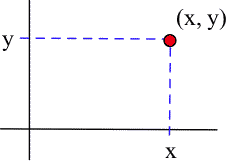
\includegraphics[width=0.4\textwidth]{img/chap4/image002.png}
    \caption{A point in the $xy$-plane.}
    \label{fig:4-1-2dPoint}
\end{figure}
Each ordered pair $(x,y)$ specifies the location of exactly one point, and the location of each point is given by exactly one ordered pair $(x,y)$. The $x$ and $y$ values are the coordinates of the point $(x,y)$.

The situation in three dimensions is very similar. In the 3-dimensional rectangular coordinate system we have three coordinate axes that meet at right angles, and three numbers, an ordered triple $(x,y,z)$, are needed to specify the location of a point.

\begin{figure}[!ht]
  \centering
    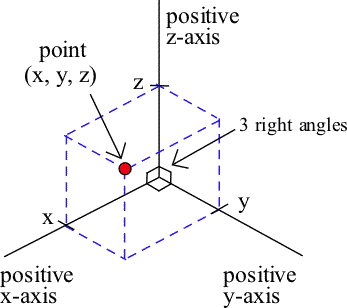
\includegraphics[width=0.4\textwidth]{img/chap4/image003.png}
    \caption{A point in 3-dimensional space.}
    \label{fig:4-1-3dPoint}
\end{figure}
Each ordered triple $(x,y,z)$ specifies the location of exactly one point, and the location of each point is given by exactly one ordered triple $(x,y,z)$. The $x$, $y$, and $z$ values are the coordinates of the point $(x,y,z)$. Figure \ref{fig:4-1-Point423} shows the location of the point $(4, 2, 3)$.

\begin{figure}[!ht]
  \centering
    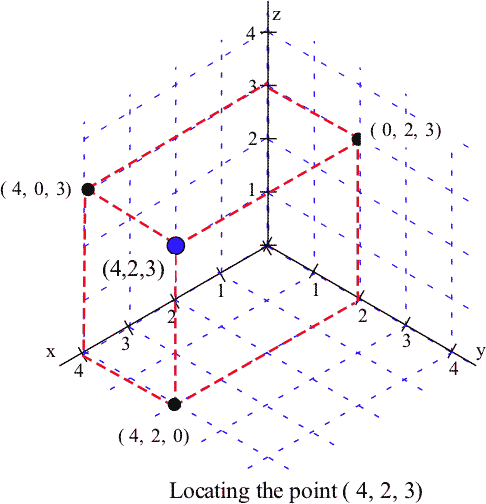
\includegraphics[width=0.4\textwidth]{img/chap4/image004.png}
    \caption{Locating the point $(4,2,3)$}
    \label{fig:4-1-Point423}
\end{figure}

Typically we use a {\bf right-hand orientation}\index{Right-hand rule}. To see what this means, imagine your right hand in front hand in front of you with the palm toward your face, your thumb pointing up, you index finger straight out, and your next finger toward your face (and the two bottom fingers bent into the palm). Then, in the right hand coordinate system, your thumb points along the positive $z$-axis, your index finger along the positive $x$-axis, and the other finger along the positive $y$-axis. See Figure \ref{fig:4-1-hand}

\begin{figure}[!ht]
  \centering
    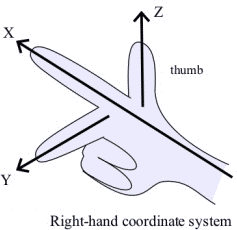
\includegraphics[width=0.4\textwidth]{img/chap4/image005.png}
    \caption{The right-hand rule for 3-dimensional coordinates}
    \label{fig:4-1-hand}
\end{figure}
Other orientations of the axes are possible and valid (with appropriate labeling), but the right-hand system is the most common orientation and is the one we will generally use. If another orientation is used, then the axes will be explicitly labeled.

Each ordered triple $(x,y,z)$ specifies the location of a single point, and this location point can be plotted by locating the point $(x,y,0)$ on the $xy$-plane and then going up $z$ units (the red path in Figure \ref{fig:4-1-3dPoint2}).

\begin{figure}[!ht]
  \centering
    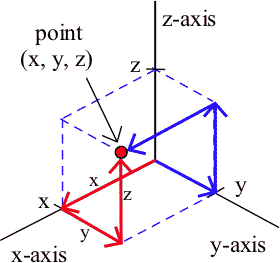
\includegraphics[width=0.4\textwidth]{img/chap4/image006.png}
    \caption{Plotting a point in 3-dimensional space}
    \label{fig:4-1-3dPoint2}
\end{figure}
We could also get to the same $(x,y,z)$ point in other ways. For instance, we could start by finding the point $(x,0,z)$ on the $xz$-plane and then going $y$ units parallel to the $y$-axis, or by finding $(0,y,z)$ on the $yz$-plane and then going $x$ units parallel to the $x$-axis (the blue path in Figure \ref{fig:4-1-3dPoint2}).

\begin{example}
Plot the locations of the points
\begin{itemize}
    \item $P=(0,3,4)$,
    \item $Q=(2,0,4)$,
    \item $R=(1,4,0)$,
    \item $S=(3,2,1)$, and
    \item $T=(-1,2,1)$.
\end{itemize}
\begin{solution} The points are shown in Figure \ref{fig:4-1-example6}.

  \begin{figure}[!ht]
    \centering
      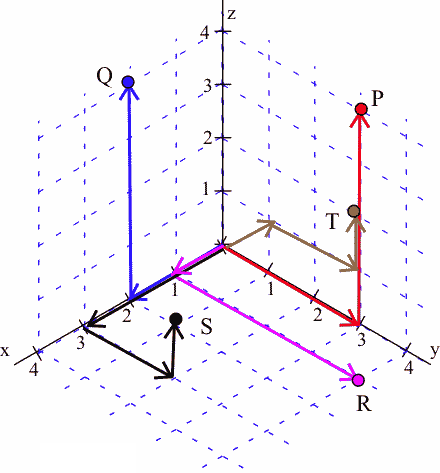
\includegraphics[width=0.4\textwidth]{img/chap4/image007.png}
      \caption{Points $P$, $Q$, $R$, $S$, and $T$}
      \label{fig:4-1-ex6}
  \end{figure}
\end{solution}\end{example}

Once we can locate points, we can begin to consider the graphs of various collections of points. By the graph of $z=2$ we mean the collection of all points $(x,y,z)$ which have the form $(x,y,2)$. Since no condition is imposed on the $x$ and $y$ variables, they take all possible values. The graph of $z=2$ is a plane parallel to the $xy$-plane and 2 units above the $xy$-plane. Similarly, the graph of $y=3$ is a plane parallel to the $xz$-plane, and $x=4$ is a plane parallel to the $yz$-plane. (Note: The planes have been drawn as rectangles in Figures \ref{fig:4-1-z2} and \ref{fig:4-1-y3x4}, but they actually extend infinitely far.)
\begin{figure}[!ht]
  \centering
    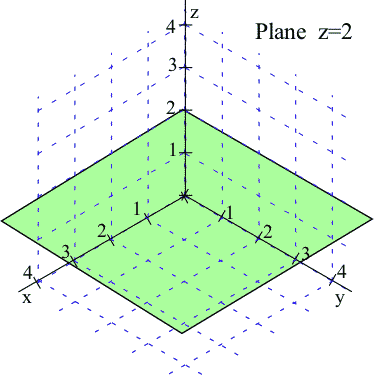
\includegraphics[width=0.4\textwidth]{img/chap4/image008.png}
    \caption{Plane $z=2$}
    \label{fig:4-1-z2}
\end{figure}
\begin{figure}[!ht]
  \centering
    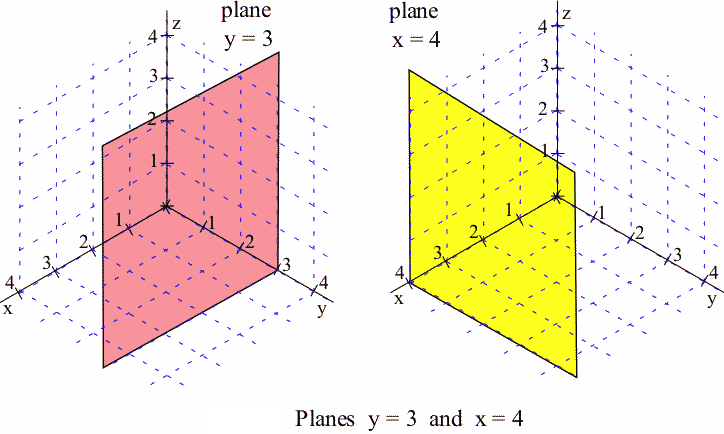
\includegraphics[width=0.8\textwidth]{img/chap4/image009.png}
    \caption{Planes $y=3$ and $x=4$}
    \label{fig:4-1-y3x4}
\end{figure}

\paragraph*{Distance Between Points}
In two dimensions we can think of the distance between points as the length of the hypotenuse of a right triangle, and that leads to the Pythagorean formula:
$$\mbox{distance} = \sqrt{(\Delta x)^2 + (\Delta y)^2 } \enspace .$$
\begin{figure}[!ht]
  \centering
    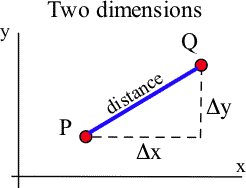
\includegraphics[width=0.4\textwidth]{img/chap4/image010.png}
    \caption{Distance in two dimensions}
    \label{fig:4-1-2dDist}
\end{figure}
In three dimensions we can also think of the distance between points as the length of the hypotenuse of a right triangle.

\begin{figure}[!ht]
  \centering
    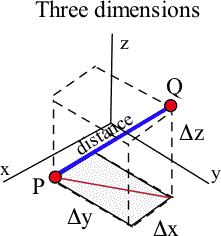
\includegraphics[width=0.4\textwidth]{img/chap4/image011.png}
    \caption{Distance in three dimensions}
    \label{fig:4-1-3dDist}
\end{figure}
In this situation the calculations may appear more complicated, but they are straightforward and the final formula is what we hope it would be given the 2-dimensional formula:
\begin{align*}
    \mbox{distance}^2   &= \mbox{base}^2 + \mbox{height}^2 \\
                        &= \left(\sqrt{(\Delta x)^2 + (\Delta y)^2}\right)^2 + (\Delta z)^2\\
                        &= (\Delta x)^2 + (\Delta y)^2 + (\Delta z)^2 \enspace ,
\end{align*}
so
    $$\mbox{distance} = \sqrt{(\Delta x)^2 + (\Delta y)^2 + (\Delta z)^2} \enspace .$$

\begin{theorem}[Distance in 3-Dimensions]
If $P=(x_1,y_1,z_1)$ and $Q=(x_2,y_2,z_2)$ are points in space, then the distance between $P$ and $Q$ is
\begin{align*}
\mbox{distance} &= \sqrt{(\Delta x)^2 + (\Delta y)^2 + (\Delta z)^2} \\
                &= \sqrt{(x_2-x_1)^2 + (y_2-y_1)^2 + (z_2-z_1)^2}
\end{align*}
\end{theorem}

The 3-dimensional pattern is very similar to the 2-dimensional pattern with the additional piece $\Delta z)^2$.

\begin{example}
Find the distances between points $A=(1,2,3)$ and $B=(7,5,-3$).

\begin{solution}
  $$\mbox{Dist}(A,B) = \sqrt{6^2+3^2+(-6)^2} = \sqrt{36+9+36} = \sqrt{81} = 9 \enspace .$$
\end{solution}\end{example}

In two dimensions, the set of points at a fixed distance from a given point is a circle, and we used the distance formula to determine equations describing circles: the circle with center $(2, 3)$ and radius 5 is given by $(x-2)^2 + (y-3)^2 = 5^2$ or $x^2+y^2-4x-6y = 12$.

\begin{figure}[!ht]
  \centering
    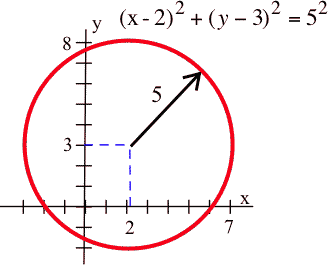
\includegraphics[width=0.4\textwidth]{img/chap4/image012.png}
    \caption{$(x-2)^2+(y-3)^2 = 25$}
    \label{fig:4-1-circle}
\end{figure}
The same ideas work for spheres in three dimensions.

\begin{definition}[Sphere]
The set of points $(x,y,z)$ at a fixed distance $r$ from a point $(a,b,c)$ is a {\bf sphere} with center $(a,b,c)$ and radius $r$.

\begin{figure}[!ht]
  \centering
    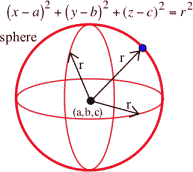
\includegraphics[width=0.4\textwidth]{img/chap4/image013.png}
    \caption{$(x-a)^2+(y-b)^2+(z-c)^2 = r^2$}
    \label{fig:4-1-sphere}
\end{figure}
The sphere is given by the equation
$$(x-a)^2+(y-b)^2+(z-c)^2=r^2 \enspace .$$
\end{definition}

\begin{example}
Write the equations of a sphere with center $(2, -3, 4)$ and radius 3.

\begin{solution} The equation is
$$(x-2)^2+(y+3)^2+(z-4)^2=3^2=9.$$
\end{solution}\end{example}

Now suppose that we want to graph a surface. We can think of each input $(x,y)$ as a location on the plane, and plot the point $f(x,y)$ units above that point. Graphing that can be challenging. We have a few options:
  \begin{itemize}
    \item Use a computer program (such as GeoGebra or SageMath) to draw beautiful perspective drawings.

\begin{figure}[!ht]
  \centering
    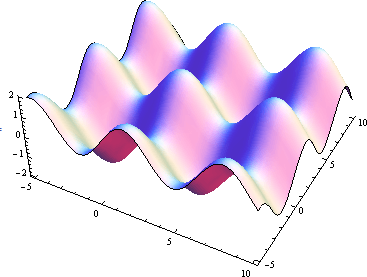
\includegraphics[width=0.4\textwidth]{img/chap4/image014.png}
    \caption{Surface}
    \label{fig:4-1-surface}
  \end{figure}
If such a program is available, then this is usually the most accurate option.

  \item Try to draw a perspective drawing by hand. This is very challenging, and usually not worth the effort.
  \item Use level curves to draw contour diagrams (or contour maps), which is the approach we'll focus on here. A contour diagram is like a topographical map -- points with the same elevation (outputs) are connected with curves. Each particular output is called a level, and these curves are called {\bf level curves}\index{Level curve} or {\bf contours}\index{Contour}. The closer the curves are to each other, the steeper that section of the surface. Topographical maps give hikers information about elevation, steep and shallow grades, peaks and valleys. Contour diagrams give us the same kind of information about a function.
\end{itemize}
Figure \ref{fig:4-1-contour1} is a contour diagram of the same surface shown in Figure \ref{fig:4-1-surface}. The level curves are graphs in the $xy$-plane of curves $f(x,y)=c$ for various constants $c$.

\begin{figure}[!ht]
  \centering
    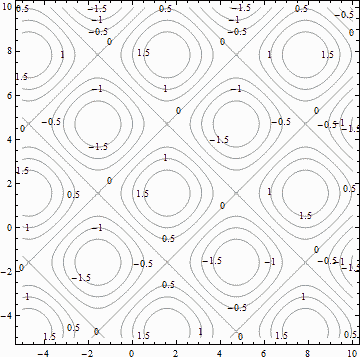
\includegraphics[width=0.4\textwidth]{img/chap4/image015.png}
    \caption{Contour map}
    \label{fig:4-1-contour1}
  \end{figure}
Each of the squares in Figure \ref{fig:4-1-contour1} corresponds to one of the bumps on the surface. If the contours are positive, as highlighted in Figure \ref{fig:4-1-contour2}, the bump is above the $xy$-plane. If the contours are negative, the bump extends below the $xy$-plane.

\begin{figure}[!ht]
  \centering
    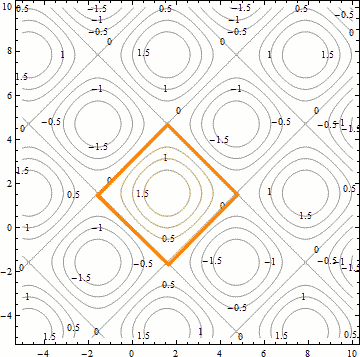
\includegraphics[width=0.4\textwidth]{img/chap4/image016.png}
    \caption{Contour map}
    \label{fig:4-1-contour2}
  \end{figure}
Everywhere on the crisscrossed pattern of diagonal lines, the height of the surface is 0, so the surface is on the $xy$-plane. This is a feature that we wouldn't necessarily have seen when we looked at the perspective drawing. Contour maps can help us see features of the surface that the 3-dimensional graph doesn't show.

\begin{figure}[!ht]
  \centering
    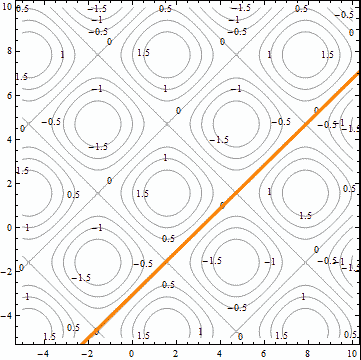
\includegraphics[width=0.4\textwidth]{img/chap4/image017.png}
    \caption{Contour map}
    \label{fig:4-1-contour3}
  \end{figure}
To better understand contour diagrams, suppose we had a table of elevation data. We could graph this by plotting the height at each point and connecting the dots with smooth curves, which would result in the something like the graph shown in Figure \ref{fig:4-1-surface2}

\begin{figure}[!ht]
  \centering
    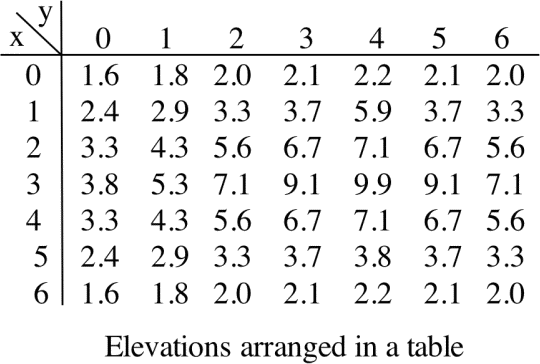
\includegraphics[width=0.4\textwidth]{img/chap4/image018.png}
    %\caption{Contour map}
    %\label{fig:4-1-contour3}
  \end{figure}
  \begin{figure}[!ht]
    \centering
      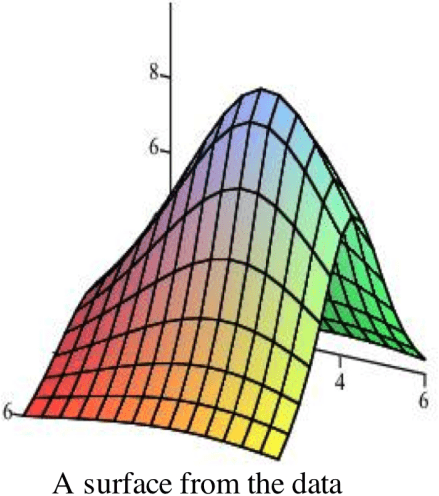
\includegraphics[width=0.4\textwidth]{img/chap4/image019.png}
      \caption{Surface from the data}
      \label{fig:4-1-surface2}
    \end{figure}
If we slice the surface in Figure \ref{fig:4-1-surface2} with the plane $z=8$, the points where the plane cuts the surface are those points where the elevation of the surface is 8 units above the $xy$-plane. Figure \ref{fig:4-1-surfaceSlice} shows the surface being sliced by the planes $z=8$ and $z=4$. Slicing the surface at different elevations and sketching the curves where the plane intersects the surface results in the graph in Figure \ref{fig:4-1-surfaceSlice2}.

\begin{figure}[!ht]
  \centering
    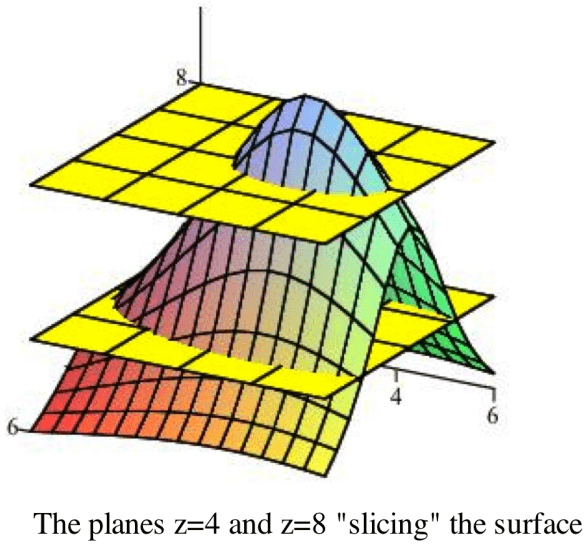
\includegraphics[width=0.4\textwidth]{img/chap4/image020.png}
    \caption{Slices of the surface}
    \label{fig:4-1-surfaceSlice}
  \end{figure}\begin{figure}[!ht]
    \centering
      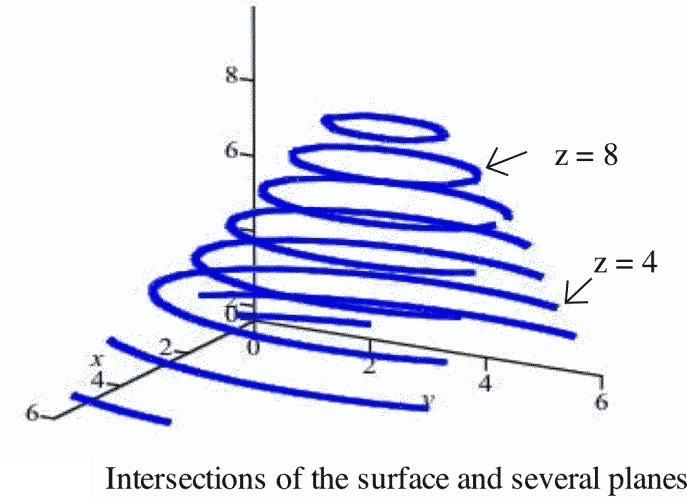
\includegraphics[width=0.4\textwidth]{img/chap4/image021.png}
      \caption{Slices of the surface}
      \label{fig:4-1-surfaceSlice2}
    \end{figure}
If we move all of those curves to the $xy$-plane (or, equivalently, view them from directly overhead), the result is a 2-dimensional graph of the level curves of the original surface. This is the contour diagram in Figure \ref{fig:4-1-contour4}.

\begin{figure}[!ht]
  \centering
    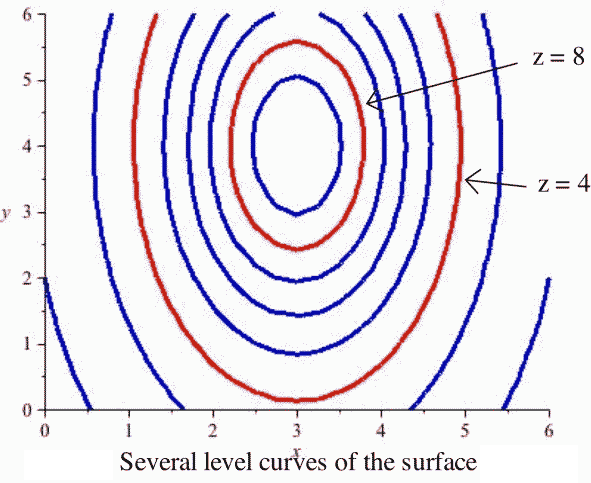
\includegraphics[width=0.4\textwidth]{img/chap4/image022.png}
    \caption{Level curves of the surface}
    \label{fig:4-1-contour4}
  \end{figure}
\begin{example}
Create a contour diagram for our car rental example with cost function $C(d,m)=40d+0.15m$. Draw curves for when the cost is 0, 100, 200, 300, and 400.

\begin{solution}
  We'll set $C(d,m)=40d+0.15m=c$ for $c = 0$, 100, 200, 300, and 400 and draw the curves in the $dm$-plane.

The first coordinate of the ordered pair is $d$, so the $d$-axis will be horizontal; the $m$-axis will be vertical. Remember that the domain for this function is really just where $d \geq 0$ and $m \geq 0$, so we will only draw the curves in the first quadrant.

When $c=0$:
\begin{align*}
C(d,m)  &= 40d + 0.15m = 0 \\
0.15m   &= -40d \\
m       &= \frac{40}{0.15}d \approx   -267d
\end{align*}
This is the equation of a line, with slope about $-267$, passing through the origin. Because of the domain restrictions, the curve we will draw for this level is simply the origin. Putting this back into the car rental context, the only point where we pay \$0 for renting the car is when we rent the car for 0 days and drive it 0 miles -- that is, if we don't rent it at all.

When $c=100$:
\begin{align*}
C(d,m) = 40d + 0.15m &= 100 \\
    0.15m &= -40d+100 \\
    m &= -\frac{40}{0.15}d + \frac{100}{0.15}\approx   -267d+667
\end{align*}
This is the equation of a line, with slope about $-267$, and $d$-intercept of about 667. This section of this line that lies in the first quadrant is shown with 100 labeling it.

Putting this into context, any point on that line represents a $(d,m)$ combination of days and miles that will make the cost exactly \$100. So, for example -- if we rent the car for 0 days and drive it 667 miles, it will cost us \$100. If we rent the car for 2.5 days and don't drive it at all, it will cost us \$100.

We continue for $c= 200, 300$, and 400 and sketch the curves in the plane, resulting in the contour diagram shown in Figure \ref{fig:4-1-contour5}.

\begin{figure}[!ht]
  \centering
    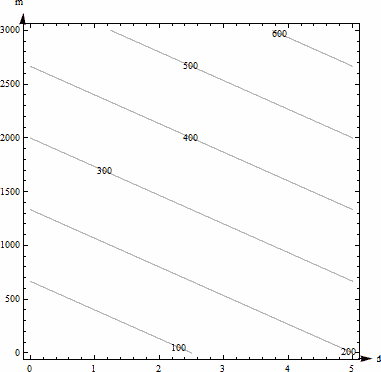
\includegraphics[width=0.4\textwidth]{img/chap4/image023.png}
    \caption{Level curves of $C(d,m) = 40d + 0.15m$}
    \label{fig:4-1-contour5}
  \end{figure}
\end{solution}\end{example}

\begin{example}
The contour diagram for the cost $C(d,m)$ in dollars for renting a car for d days and driving it m miles is shown in the previous example. Use the diagram to answer the following questions.
\begin{enumerate}[label=(\alph*)]
    \item What is the cost of renting a car for 3 days and driving it 200 miles?

    \begin{solution} The point $(3, 200)$ is between contours on this graph, so we can’t get an exact answer for $C(3,200)$. (But it’s typical for a graph that we would have to estimate). It looks to me as if $(3, 200)$ is halfway between the 100 and the 200 contours, so let's estimate that $C(3,200)$ is about \$150.

Estimates from the graph are necessarily very rough. The graph only shows a little information (in this way, a contour diagram is like a table), so we have to extrapolate in between. But for most graphs, we don’t actually know what happens between the contours. All we know for sure is that the output at $(3, 200)$ is between the two levels we see. For this car rental example, we also know a formula, and my table showed this particular input, so we have other ways to get a better answer.
    \end{solution}
    \item What is $C(100,4)$? What is $C(4,100)$?

    \begin{solution} We can't find $(100, 4)$ on this diagram, so we can't make an estimate of $C(100,4)$ from this graph. $(4, 100)$ lies between the contours for 100 and 200. It looks closer to 200, so let's estimate that $C(4,100)$ is about \$180.
    \end{solution}
    \item Suppose we rent the car for 3 days. Is $C$ an increasing function of miles?

    \begin{solution} If we fix $d=3$, we get a vertical line. What happens as $m$ increases on this vertical line? As $m$ increases, the function values shown on the contours increase, so $C$ appears to be an increasing function of miles.
    \end{solution}
\end{enumerate}
\begin{figure}[!ht]
  \centering
    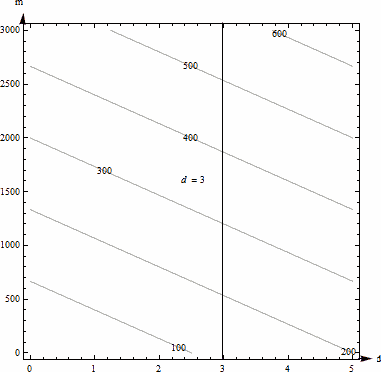
\includegraphics[width=0.4\textwidth]{img/chap4/image024.png}
    \caption{Level curves of $C(d,m) = 40d + 0.15m$ with $d=3$}
    \label{fig:4-1-contour6}
  \end{figure}
\end{example}

\begin{example}
Here is a contour diagram for a function $g(x,y)$.

\begin{figure}[!ht]
  \centering
    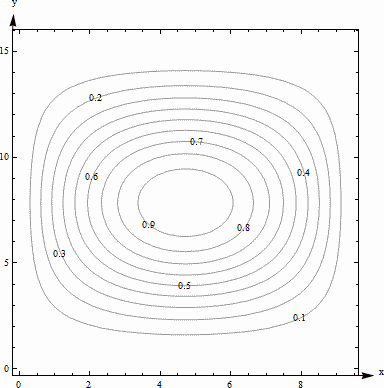
\includegraphics[width=0.4\textwidth]{img/chap4/image025.png}
    \caption{Level curves of $z=g(x, y)$}
    \label{fig:4-1-contour7}
  \end{figure}
Use Figure \ref{fig:4-1-contour7} to answer the following questions:
  \begin{enumerate}[label=(\alph*)]
    \item What is $g(3,5)$?
    \begin{solution}
    $g(3,5)$ is 0.6. We can tell because the point is right on one of the contours, as illustrated in Figure \ref{fig:4-1-contour8}.

    \begin{figure}[!ht]
      \centering
        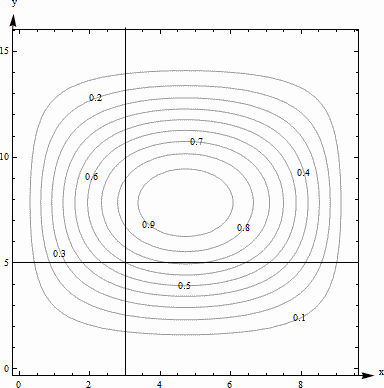
\includegraphics[width=0.4\textwidth]{img/chap4/image026.png}
        \caption{Level curves of $z=g(x, y)$ with $x=3$ and $y=5$}
        \label{fig:4-1-contour8}
      \end{figure}
    \end{solution}
    \item What is the highest point shown on the diagram? What is the lowest point shown?
    \begin{solution}
      The highest contour shown is 0.9, and there would be a contour for 1.0 if the surface had ever got that high. However, the height seems to be increasing as we move in toward the center, so it appears that g gets to nearly 1 in the center. The lowest contour is 0.1. But again, we will guess that the height continues to decrease, so it appears that $g$ is nearly 0 around the outside.
    \end{solution}
    \item If you start at $(3, 5)$ and head in the positive $x$ direction, do you go uphill or downhill first?
    \begin{solution}
      Starting at the point $(3, 5, 0.6)$ on the surface and traveling to the right along the horizontal line shown in the previous part, we would cross the contour for 0.7 next. So the function increases first (we go uphill), and then decreases again.
    \end{solution}
  \end{enumerate}
Again, remember that we don't really know what happens between the contours. All we can do is estimate from the information in the graph.
\end{example}

\begin{example}
Here is a contour diagram for a function $F(x,y)$.

\begin{figure}[!ht]
  \centering
    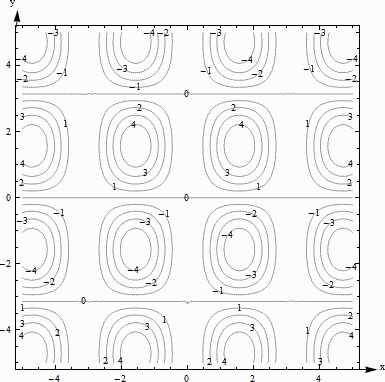
\includegraphics[width=0.4\textwidth]{img/chap4/image027.png}
    \caption{Level curves of $z=F(x, y)$}
    \label{fig:4-1-contour9}
  \end{figure}
  \begin{enumerate}[label=(\alph*)]
    \item Describe the shape of the surface.
    \begin{solution}
      The surface is bumpy, with regularly spaced oval bumps. Notice that some of the bumps go up (positive contours), but others go down. Between the bumps, there are horizontal lines that are completely level, with an elevation of 0.
    \end{solution}
    \item Suppose you travel along the surface in the positive $y$-direction, starting on the surface at the point above (or below) the point $(x,y)=(-1,1)$. Describe your journey.
    \begin{solution}
      It looks as if $F(-1,1)$ is about 3. As we head in the positive $y$-direction along the line shown in Figure \ref{fig:4-1-contour10}, we first go uphill, nearly to 4, then we start going downhill. As we keep going north, we keep descending, going into the dip, until nearly $-4$. We're starting to go uphill again just as we leave the graph.

      \begin{figure}[!ht]
        \centering
          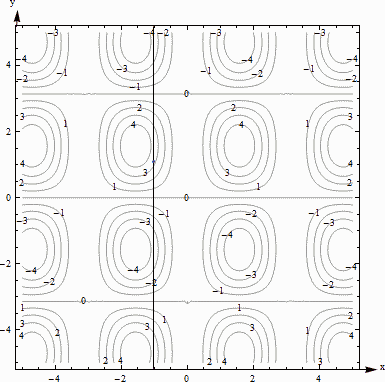
\includegraphics[width=0.4\textwidth]{img/chap4/image028.png}
          \caption{Level curves of $z=F(x, y)$ with $x=-1$}
          \label{fig:4-1-contour10}
        \end{figure}
      \end{solution}
    \end{enumerate}
\end{example}

What happens if you have a function of more than two variables? Its graph will be a {\bf hyper-surface}\index{Hyper-surface}. For example, the graph of a function of four variables will be a hyper-surface in 5-dimensional space. This is very difficult (impossible for most of us) to visualize. Even the contours are hard to visualize -- instead of curves in the plane, they're hyper-surfaces in 4-dimensional space. So if you have more than two variables, the graph isn't usually very useful.

%Functions of Two Real-Life Variables
\subsection{Complementary Goods and Substitute Goods}
The demand for some pairs of goods have a relationship, where the quantity demanded for one product depends somehow on the prices for both
\begin{definition}[Complementary Goods]
Two goods are {\bf complementary}\index{complimentary goods} if an increase in the price of either decreases the demand for both.
\end{definition}

\begin{example} Here are two examples of complementary goods.
\begin{itemize}
  \item The demand for cars depends on both the price for cars and the price of gasoline.
  \item The demand for hot dog buns depends on both the price for the buns and the price for the hot dogs.
\end{itemize}
\end{example}

\begin{definition}[Substitute Goods]
Two goods are {\bf substitutes} if an increase in the price of one increases the demand for the other.
\end{definition}
\begin{example} Here is an example of substitute goods.
\begin{itemize}
  \item The demand for Brand A depends on its price and also on the price of its main competitor Brand B. If the Brand B raises its price, consumers will switch brands (substitute) and demand for Brand A will increase.
\end{itemize}
\end{example}
Think about brands of soft drinks, detergent, or paper towels. A traditional example is coffee and tea: the idea is that consumers are simply looking for a hot drink and they'll buy whatever is cheaper. But this has always seemed fishy to me -- I've never met any coffee- or tea-drinkers who would happily switch.

These demand functions are functions of two variables.

\begin{example}
The demand functions for two products are given below. $p_1$, $p_2$, $q_1$, and $q_2$ are the prices (in dollars) and quantities for Products 1 and 2:
\begin{align*}
q_1 &= 200-3p_1-p_2\\
q_2 &= 150-p_1-2p_2
\end{align*}
Are these two products complementary goods or substitute goods? What is the quantity demanded for each when the price for Product 1 is \$20 per item and the price for Product 2 is \$30 per item?

\begin{solution} These products are complementary: an increase in either price decreases both demands. You can see that because the coefficients are both negative in each demand function.

When $p_1=20$ and $p_2=30$, we have
\begin{align*}
q_1 &= 200-3(20)-(30)=110\\
q_2 &= 150-(20)-2(30)=70
\end{align*}
So 110 units are demanded for Product 1 and 70 units are demanded for Product 2 when the price for Product 1 is \$20 per item and the price for Product 2 is \$30 per item.
\end{solution}\end{example}

\subsection{Cobb-Douglas Production Function}
\label{ssec:cobb-douglas}
Production functions are used to model the total output of a firm for a variety of inputs (doesn't this sound like a function of several variables?). One example is a {\bf Cobb-Douglas Production function}\index{Cobb-Douglas Production function}:
$$P=AL^{\alpha}K^{\beta} \enspace ,$$
where $P$ is the total production, $A$ is a constant, $\alpha$ and $\beta$ are constants between 0 and 1, $L$ is the labor force, and $K$ is the capital expenditure. (The units must be massaged well.)

You can read more about Cobb-Douglas Production functions at \url{http://en.wikipedia.org/wiki/Cobb-Douglas}. You can read about other kinds of production functions at \url{http://en.wikipedia.org/wiki/Production_function}.
